\section{\acs*{vbl} methods}

In the previous section, we have described data representation mostly used in \ac{vbl}. The current section is dedicated to the method built on this representation to perform localization. As mentioned in the introduction, it exists two main family of methods:
\begin{itemize}
	\item \Acf{cbir} for localization,
	\item 6 \ac{dof} camera pose estimation.
\end{itemize}

We can mention a last and recent family of \ac{vbl} method, named coarse to find localization, that can be seen as a combination of the two aforementioned localization systems.
\label{sec:vbl_methods}
	
\subsection{\acs*{cbir} for localization}
\begin{figure}[t]
	\centering

	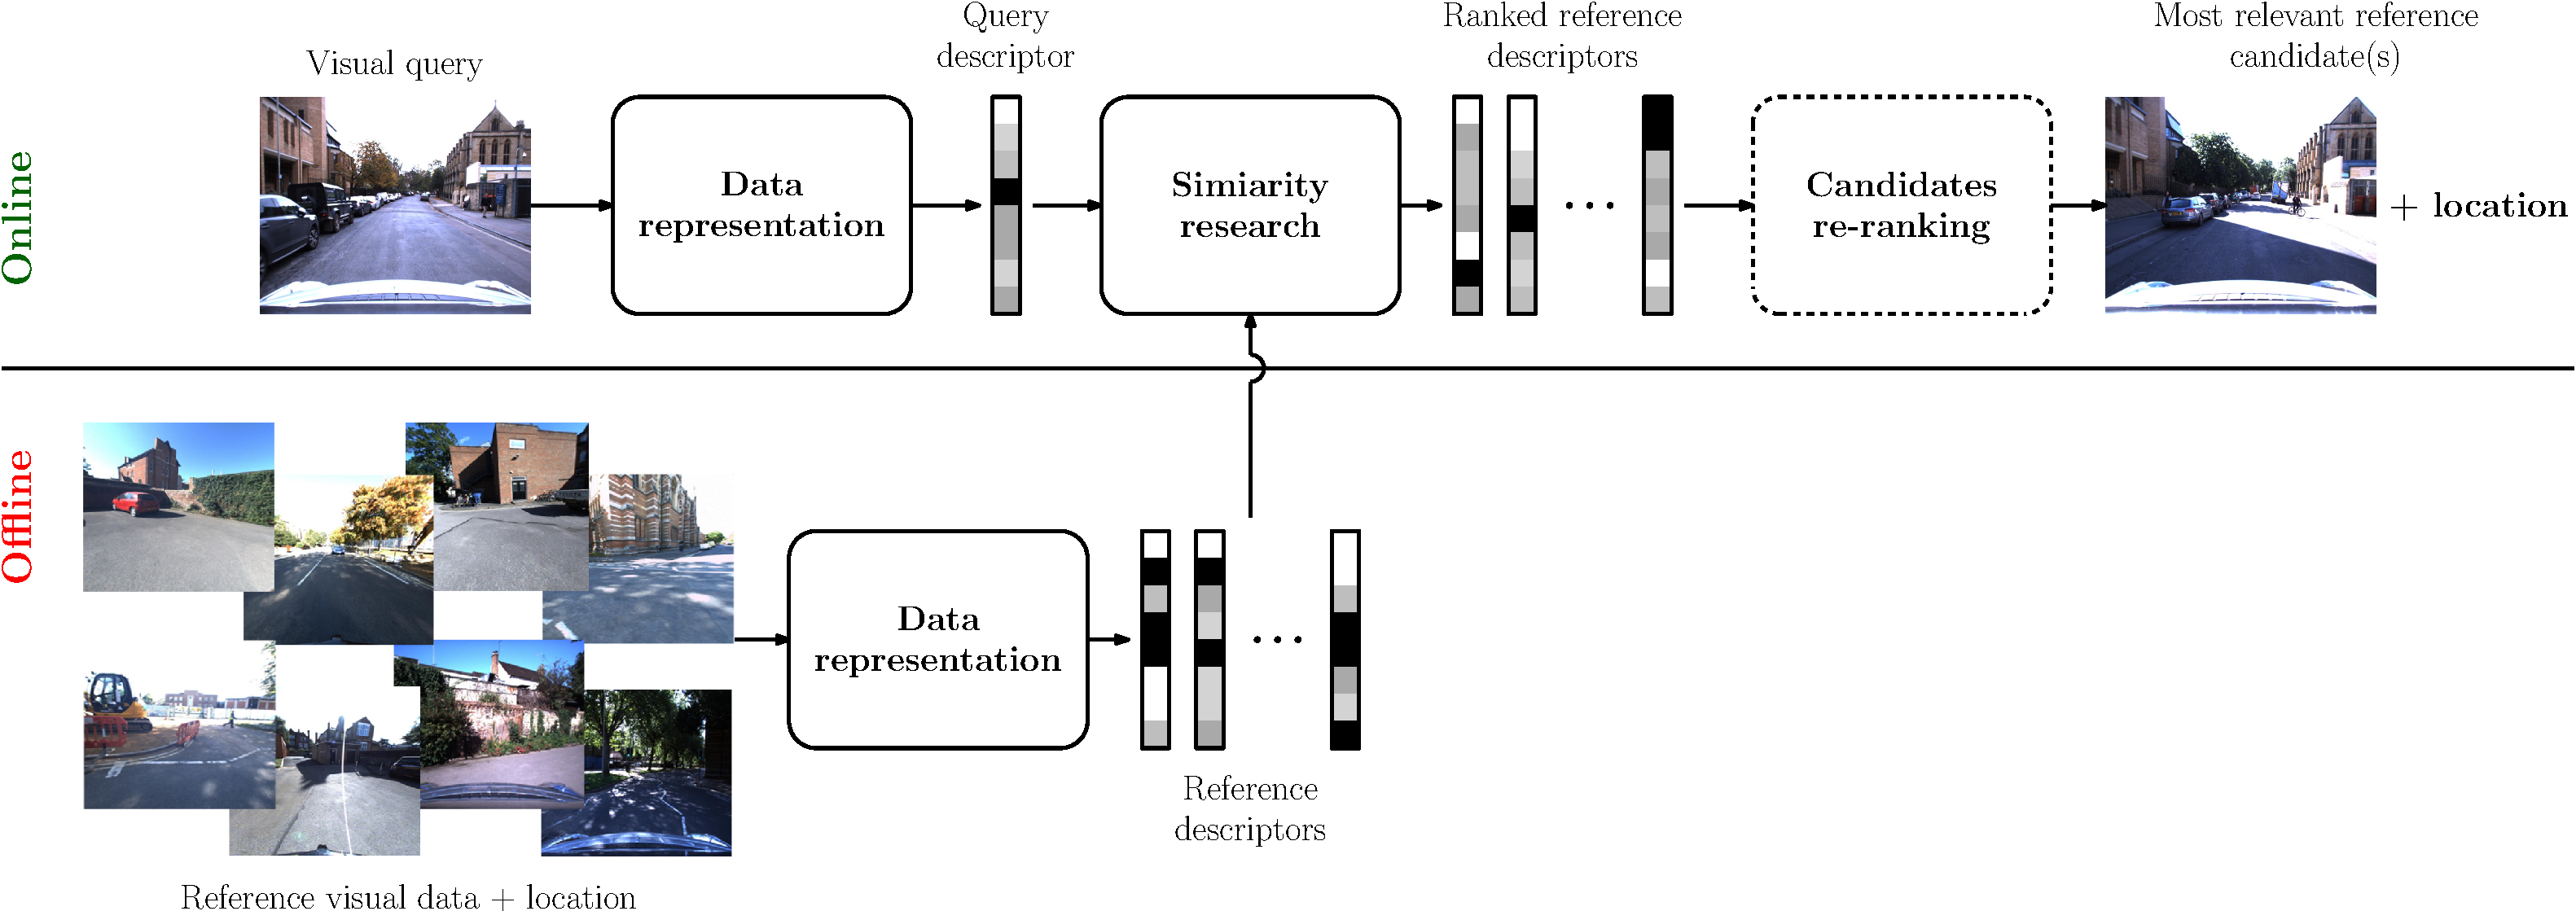
\includegraphics[width=\linewidth]{methods/cbir_for_localization}
	\caption[CBIR for localization]{\label{fig:cbir_for_localization}\textbf{CBIR for localization:} the location of a given request can be retrieved by comparing the query to a pool of geolocalized candidates. After the similarity comparison, the location associated to the top-ranked reference data is considered as the location of the query. Re-ranking of the reference data can be used in order to improve the relevance of the top-ranked candidates.}
\end{figure}


\label{subsec:vbl_as_image_retrieval}
The aim of \ac{cbir} methods is to retrieve a set of data presents in the database that are similar to an input query. This is a problem related to instance retrieval~\citep{Zheng2017}. As the visual data used in \ac{vbl} are augmented with geospatial information (\textit{e.g.} a geotag associated to an image), retrieving documents comparable to the input provides an information on the possible location of the query. This localization method is three-step: description of the visual data, similarity association across the description vectors previously extracted and possible candidates re-ranking. \acs*{cbir} for localization pipeline is illustrate in figure~\ref{fig:cbir_for_localization}.

\subsubsection{Efficient data representation for localization}
As one of our main contribution in this thesis targets the design of a new learned global image representation for long-term \ac{cbir} for localization, we do not detail data description in this chapter. We refer reader to the first section of \acl{chp}~\ref{chap:3}, \acs{sec}~\ref{sec:cbir_data_for_loc}, for a comprehensive review of image representation suited for localization.

For the subsequent tasks of the localization process, we assume that we are able to produce low dimensional vectors to describe the visual data.

\subsubsection{Similarity Research}
\label{subsubsec:similarity_research}

The similarity research step involve evaluating the sameness between the request descriptor (\ie the description vector computed from the visual request we want to localize) and the reference descriptors. At the end of this step, we obtain a list of reference candidates, ranked accordingly to their similarity to the request.

\paragraph{Pre-processing.}
Dimension reduction of descriptor is often performed to reduce matching time and memory footprint. The most used technique remains the \ac{pca}. \ac{pca} is applied on hight dimension vector, \textit{e.g.} weights extracted from CNN layers (\citep{Arandjelovic2017,Gordo2016}). \ac{pca} has also been used to reduce the size of local features aggregated vectors \citep{Kim2015,Torii2015} or global descriptors \citep{Ni2009}. Gaussian Random Projection is applied in~\citep{Sunderhauf2015a,Panphattarasap2016} and in a different work, binary locality-sensitive hashing~\citep{Sunderhauf2015} is used instead. To reinforce data consistency, whitening could be applied to final features before the similarity search~\citep{Jegou2012a,Gong2014,Tolias2016,Arandjelovic2017,Gordo2016,Radenovic2016}.

\paragraph{Similarity metric.}
For most methods, comparison between descriptors is a trivial operation: it consists in a simple euclidean distance computation between vectors (with $L2$ norm or cosine similarity -- \textit{if the vectors are unitary} -- as usually used metric). Area correlation is another approach for computing data similarity. Simple forms of correlation like Sum of Squared Difference (SSD) or Sum of Absolute Difference (SAD) have been used in \ac{vbl} to directly compare raw images~\citep{Poglitsch2015,Milford2015}. \citet{Wan2016} use PC (Phase Correlation) on images described with FT (Fourier Transform) in order to be robust to shadow artifacts. In the work of~\citep{Corke2013}, authors compare shadow invariant grey-scale images with Zero Mean Normalized Cross-Correlation (ZNCC).

\paragraph{\Acl{nn} Search.}
In some works, when the amount of data to compare remain acceptable, linear or brute-force retrieval procedure can be employed to retrieve the closest neighbors. Hierarchical structures can be used in order to speed-up the research process (\eg k-d-tree). Linear \ac{nn} search is used in~\citep{Babenko2014,Sunderhauf2015,Radenovic2016,Gordo2016,Arandjelovic2017,Zamir2010,Zamir2014,Sunderhauf2015a}, among others, where low-dimension global image descriptor (\S\ref{subsec:global_feature}) are used to describe the data.

Exact nearest neighbor search becomes impracticable when the amount and/or dimensionality of the features are too large. Authors then turn to approximate nearest neighbor search to trade efficiency for rapidity, thus accepting some errors in the retrieved neighbors. Approximate matching involve hashing methods~\citep{Gionis1999}, well-suited data structure like inverted-index and quantization frameworks~\citep{Nister2006,Philbin2007,Jegou2011}. Interested readers may see~\citep{Wang2017} for more details.

Several \ac{nn} search algorithms are efficiently implemented in the \texttt{FLANN} library~\citep{Muja2009}, and in the new Facebook \texttt{FAISS} library~\citep{Johnson2017}.

\paragraph{Machine Learning matching Methods.}
Learning the distribution of the extracted features is an alternative to aforementioned \ac{nn} search methods.

\Ac{svm} classifier is used in numerous works~\citep{Shrivastava2011,Cao2013,McManus2014,Aubry2014} to cast the similarity research as a classification task. \citet{Cao2013} initially cluster the database according to the resemblance of the images. On top of this graph of similar images, they trained \ac{svm} for each cluster and at query time oppose the input image to all classifiers. By selecting the data associated to the \ac{svm} reaching the higher score of classification, this approach permits to quickly retrieve a pool of similar images. In~\citep{McManus2014,Aubry2014} authors train linear classifiers on HOG descriptors to robustly retrieve similar images that present extreme appearances changes. \citet{Aubry2014} take the advantages of \ac{lda} data representation in order to avoid expensive \ac{svm} training (like hard negative mining used in~\citep{Shrivastava2011,Kim2015}). Similarly, \citet{Kim2015} train \ac{svm} classifier to predict the robustness of extracted descriptors. This improves the matching process and reduces the number of features to compare against the database.

\citet{Lu2015} introduce a \ac{mtl} layout designed for features similarity association. Works from \citet{torralba2003context} and \citet{Ni2009} present \ac{vbl} methods that are able to localize an input query among a set of predefined places. Authors embedded the recognition process into probabilistic framework, \ac{gmm} in~\citep{torralba2003context} and epitome in~\citep{Ni2009}, trained upon images representing different areas. Such paradigms allow an easy integration of additional features (such as depth information~\citep{Ni2009}).

\paragraph{Other Matching Methods.}
\citet{Stumm2015a} introduce an innovative method based on graph matching. The visual vocabulary abstraction is employed and augmented with a graph of covisibility of the visual words in images. The graph is constructed as follows: nodes represent visual word detected in images and edges are created between two nodes if they are seen together in a same image. This formulation permits integrating geometric relations between the extracted features. Authors use a graph kernel for the similarity comparison among the query graph and the database~\citep{Stumm2015,Stumm2016}. Notice that graph-based approaches are often employed when scenes are described by spatially organized semantic clues such as office furnitures~\citep{Salas-Moreno2013} or street equipments~\citep{Ardeshir2014}.

\subsubsection{Candidates re-ranking}
\label{subsec:candidates_re_ranking}
Data can be processed after the similarity research to improve the final result. Post-processing methods are widely used to re-rank the candidate list, improving relevance of retrieved data.

\paragraph{Generic re-ranking.}
Query expansion is a post-process that re-query the database after a first retrieval step to increase the recall rate~\citep{Chum2007,Chum2011,Tolias2014}. However, increasing the recall rate is not the main concern of \ac{vbl} indirect method~\citep{Sattler2012}. Indeed, as exposed in the introduction, a perfect \ac{vbl} indirect system should retrieve at first position the closest visual document present in the database. However, more suitable top ranked candidates in the list of retrieved data could benefit to a subsequent pose estimation step~\citep{Song2016}. The \ac{vbl} system presented by \citet{Cao2013} increase the diversity of retrieved images by introducing a probabilistic re-ranking on the assumption that the first ranked candidate is not a good one and by maximizing the probability that the second one is.
\label{par:ransac}
On the other hand, geometric consistency check is often used to reject wrong matching. Relative pose between the query and the database candidates is computed by considering homography or multiple-view transformation, and candidates that produce the most consistent pose are ranked up. \citet{Philbin2007} democratize the use of spatial verification by introducing prior on the pose of the photography by assuming a top-oriented view. Authors perform spatial check hierarchically to get more flexibility between time computation and retrieval precision. The geometric transformation between the query and the candidate is usually computed with minimal algorithm embedded in random consensus, like RANSAC~\citep{Fischler1981}. There exists multiple alternatives to the classical RANSAC algorithm. PROSAC by~\citep{Chum2005}, used in~\citep{Donoser2014}, prioritize specific features during the random selection step. We can also enumerate LO-RANSAC used in~\citep{Philbin2007} and AC-RANSAC in~\citep{Qu2015,Qu2016}. Novel method F-SORT presented by \citet{Chan2016} show outstanding result both in term on matching quality and computation efficiency. Notice that these algorithms, beside improving the relevance of the retrieved candidates, can give information about the relative pose of the query. That is why numerous 6 \ac{dof} pose estimation methods, presented thereafter in \acs{sec}~\ref{subsec:fine_pose_estimation}, rely also on these techniques.

\paragraph{Specific \ac{vbl} re-ranking.}
Unlike conventional methods of object-retrieval, indirect \ac{vbl} can benefit from geo-localization information associated to the documents present in the database. As discussed earlier, this information can be used to construct structured graph for the similarity search process~\citep{Torii2011,Cao2013} or exploited to re-rank the candidates list~\citep{Zamir2010,Zamir2014,Sattler2016}. \citet{Zamir2010} introduce this geographic re-ranking after a classical image-retrieval algorithm to quickly remove irrelevant candidates. Authors go one step further in~\citep{Zamir2014} and embed the matching process within a Generalized Minimum Clique Graphs scheme to retrieve consistent candidates according to the GPS tag associated to the visual data. \citet{Sattler2016} generalize the problem of visual burstiness introduced by~\citep{Jegou2009} to a geographic level, introducing the concept of geometric burstiness. They improve the relevance of the ranked list of candidates using position and popularity meta-information of database images.

\subsection{6 \acs*{dof} pose estimation}
\label{subsec:fine_pose_estimation}

At this point, we introduce camera pose estimation methods that instantly recover the exact 6 \ac{dof} pose of the query according to a known reference. Compared to \ac{cbir} approaches, 6 \ac{dof} pose estimation methods provide a more accurate query pose to the detriment of the area coverage. From this class of methods, we consider the two following approaches:
\begin{description}
	\item[Geometric methods:] this class of methods, also known as structure-based methods, performs the global localization of the query by establishing correspondences between two-dimensional features extracted from a visual query and three-dimensional model of the environment (see figure~\ref{fig:geometric_method}).
	\item[Learned approaches:] the last considered family of algorithms are methods that learn to directly regress from an input visual data to its corresponding pose. Standard regression techniques~\citep{Shotton2013} and \ac{cnn} architecture~\citep{Kendall2015} are employed to perform this task (see figure~\ref{fig:learned_method}).
\end{description}


\subsubsection{Geometric methods}
\begin{figure}[t]
	\centering

	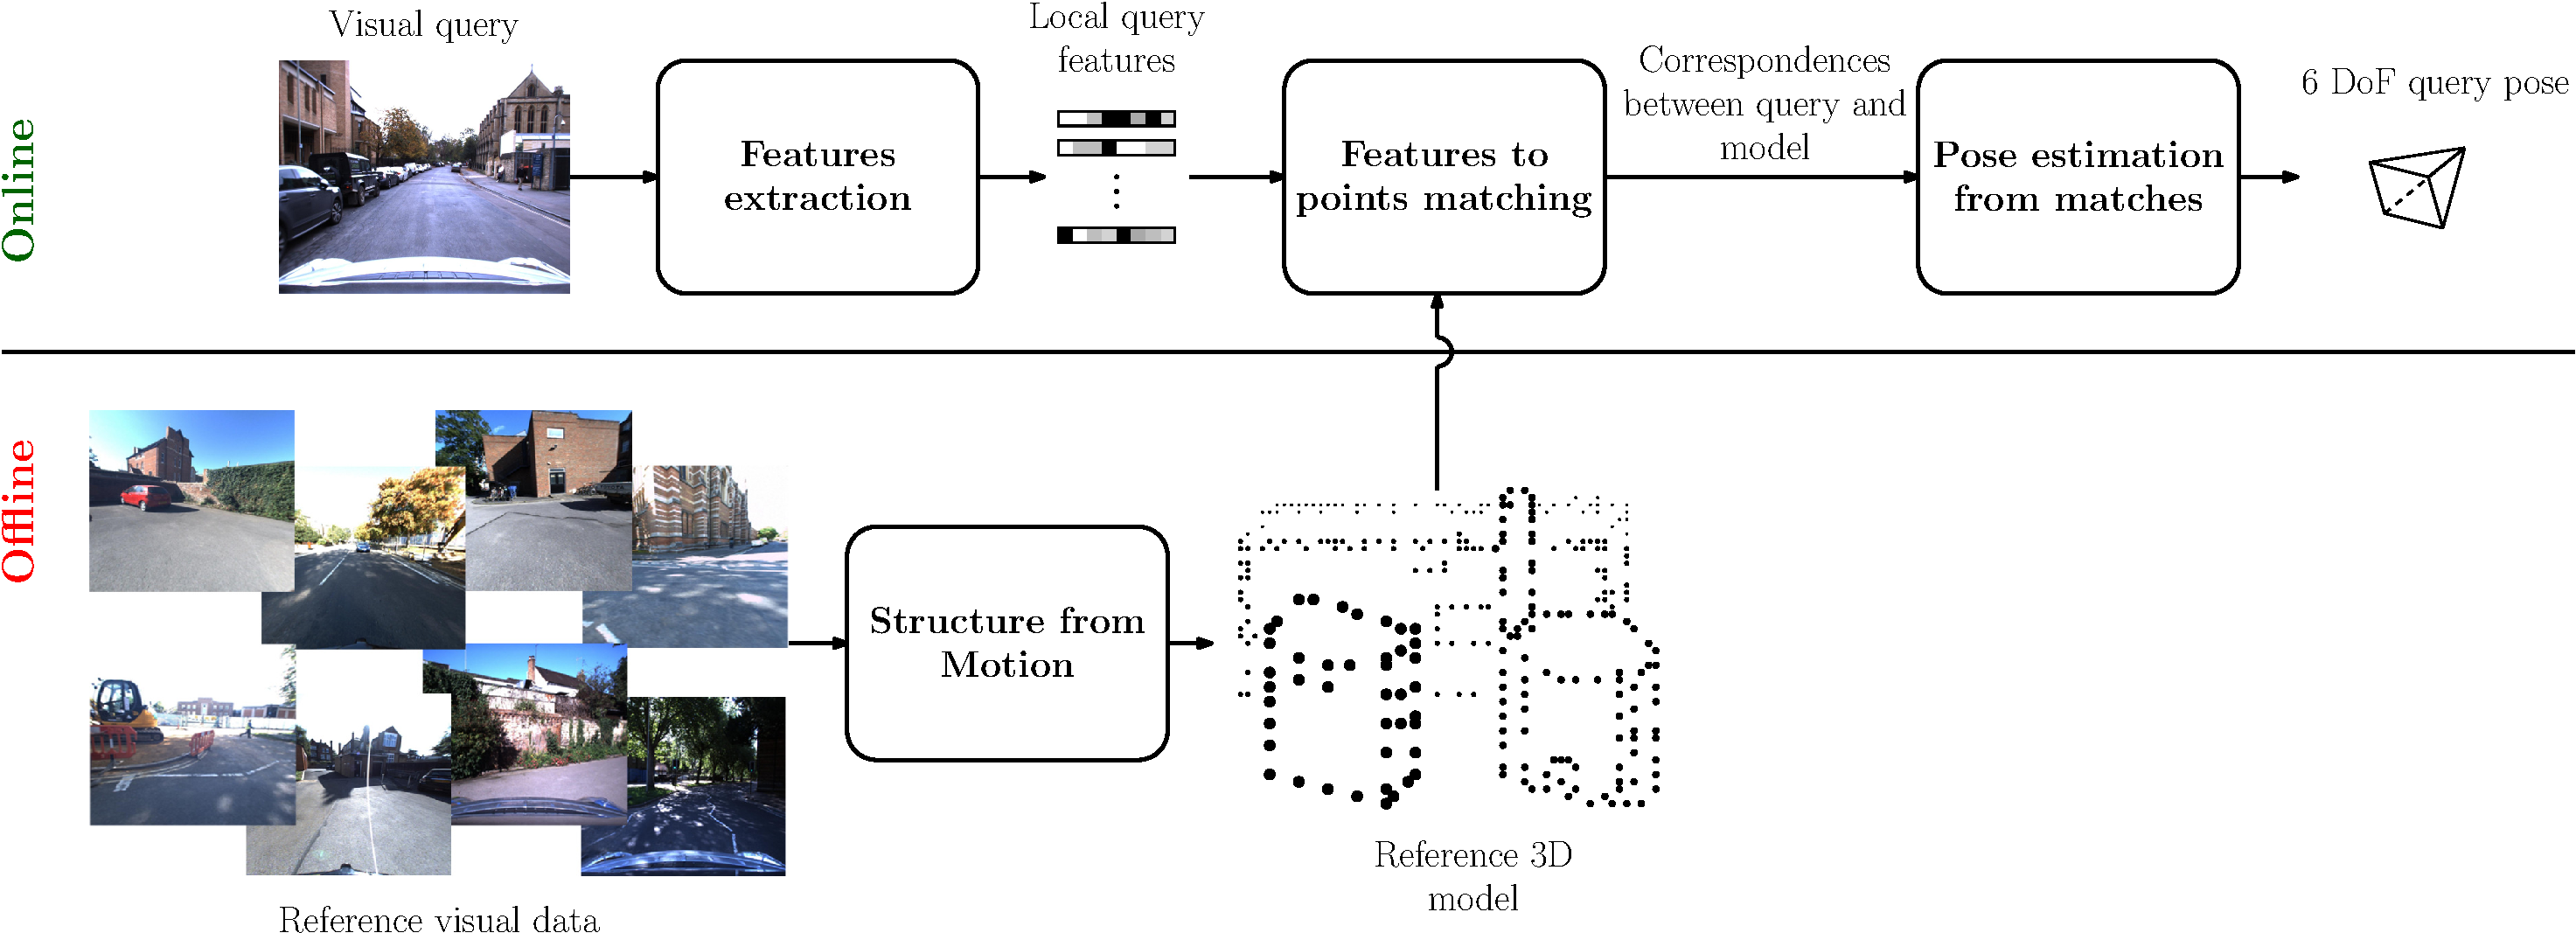
\includegraphics[width=\linewidth]{methods/geometric_method}
	\caption[Structud-based method]{\label{fig:geometric_method}\textbf{Structure-based \acs{vbl}:} reference data are used to construct a 3D model of the environment. During localization, the query is compared to this model to determine its 6-\ac{dof} pose.}
\end{figure}


\label{subsubsec:sfm_methods}
A widely represented family of \ac{vbl} methods aims to regress the pose of a camera based on the analysis of a 3D point cloud reconstructed by \ac{sfm} algorithms~\citep{schoenberger2016sfm,moulon2016openmvg,rupnik2017micmac}. The principle of these methods is to establish 2D features to 3D points correspondences (F2P). In a first step, three-dimensional representation of the environment is built thanks to many images. Triangulated points within this structure are associated to the local features (most of the time SIFT vectors~\citep{Lowe2004}) extracted from all the images where the considered point is visible. At query time, local features from the image to localize are matched against the set of pre-computed 3D points. Finally, the features to points correspondences permit a 6 \ac{dof} pose estimation of the acquisition system. The overall pipeline of structured methods is presented in figure~\ref{fig:geometric_method}.

These methods have a lot in common with \ac{cbir} for localization approaches described in Section~\ref{subsec:vbl_as_image_retrieval} as they share two major steps:~feature extraction and data association. Yet, the use of a geometrically structured database introduces interesting elements not exploitable in a classical image-retrieval scheme~\citep{Sattler2012a}.

\paragraph{Features to points matching.}
As \ac{nn} search have already been presented in the previous section\ref{subsubsec:similarity_research}, in this paragraph we focus on more specific matching methods designed for geometric \ac{vbl}.

\citet{Irschara2009} introduce the first F2P method based on \ac{sfm} environment representation. Authors perform scalable \ac{vbl} by registering the point cloud into synthetic visual documents covering the entire model. Latter improvement by \citet{Li2010} reverse the conventional process by searching from the point cloud correspondences in the image (P2F), instead of matching features from the image to points. This formulation causes an overhead in computation but is correctly handled by considering a compressed version of the \ac{sfm} model and by implementing end-conditions and rejection cases in their algorithm.

\citet{Sattler2011} consider the original features to points correspondences scheme by~\citep{Irschara2009} and introduce a Vocabulary-based Prioritized Search (VPS) inspired by BoF matching method. Subsequent works by the same authors~\citep{Sattler2012} augment the VPS framework with the points to features matching P2F~\citep{Li2010}. \citet{Li2012} show that the class of methods introduced in~\citep{Irschara2009,Li2010} can deal with large environment. Authors augment the P2F matching with hypothesis of co-occurrence of 3D points present in a close neighborhood. Based on similar spatial observation, \citet{Sattler2015} consider visibility graph to reject wrong matchings. \citet{Heisterklaus2014} introduce MPEG compression for visual document in order to speed-up the system. In the work described in~\citep{Donoser2014}, authors use the descriptor redundancy associated to 3D points to train random ferns on the top of each points. F2P matching time requirement is by the fact greatly reduced. 

Works from~\citep{Middelberg2014,Lynen2015} tackle the problem of \ac{vbl} embedded in a mobile device with limited memory storage and computational power. To achieve real-time performances, authors in~\citep{Middelberg2014} produce a very light 3D model to track the mobile camera in an urban environment. They send at regular interval key-frames to a server that is in charge of computing the global pose of the camera regarding a pre-produced point cloud. Aligning a light relative point cloud reconstructed with \ac{sfm} to a bigger one have also been investigated in~\citep{Lu2015}. \citet{Svarm2014} consider the problem of \ac{vbl} with F2P matching as a combinatorial optimization problem and design a fast outliers rejection scheme. This promising work have been improved through~\citep{Zeisl2015,Svarm2016} contributions.

State of the art strucutred methods based are dominated by techniques combining previously mentioned improvements~\citep{Sattler2016a}. Recent work by \citet{Feng2016a} reduce drastically the computational power requirement by considering fast point extractor and binary descriptors combined with an efficient similarity research. Authors show an order of magnitude in time reduction without any pose estimation performances deterioration.

\paragraph{Pose estimation.}
F2P (as well as P2D) provides correspondences between 2D pixels and 3D points. Defined by \citet{Hartley2003}, perspective-$n$-point (P$n$P) formulation is the most common tool to recover the absolute camera pose according to a point cloud reconstructed by \ac{sfm}.

Embedded in a random consensus scheme (see \S\ref{par:ransac}), six correspondences between the image and the 3D model are sufficient to retrieve the pose, if we have no information about the intrinsic parameters of the camera~\citep{Donoser2014,Li2010,Li2010,Heisterklaus2014}. This formulation is known as P6P and can be solved with Direct Linear Transformation (DLT \citep{Hartley2003}).

In particular cases, three correspondences between the image and the model are sufficient (P3P pose computation problem). Especially, the pose estimation problem can be reduced to a P3P formulation if the intrinsic parameters of the camera are known~\citep{Irschara2009,Middelberg2014}, or if 3 or more \ac{dof} are fixed~\citep{Zeisl2015,Qu2016,Svarm2016,Svarm2014}. In those particular cases, P3P solvers~\citet{Kneip2011} are mostly used to recover the pose.

\subsubsection{Learned methods}
\begin{figure}[t]
	\centering

	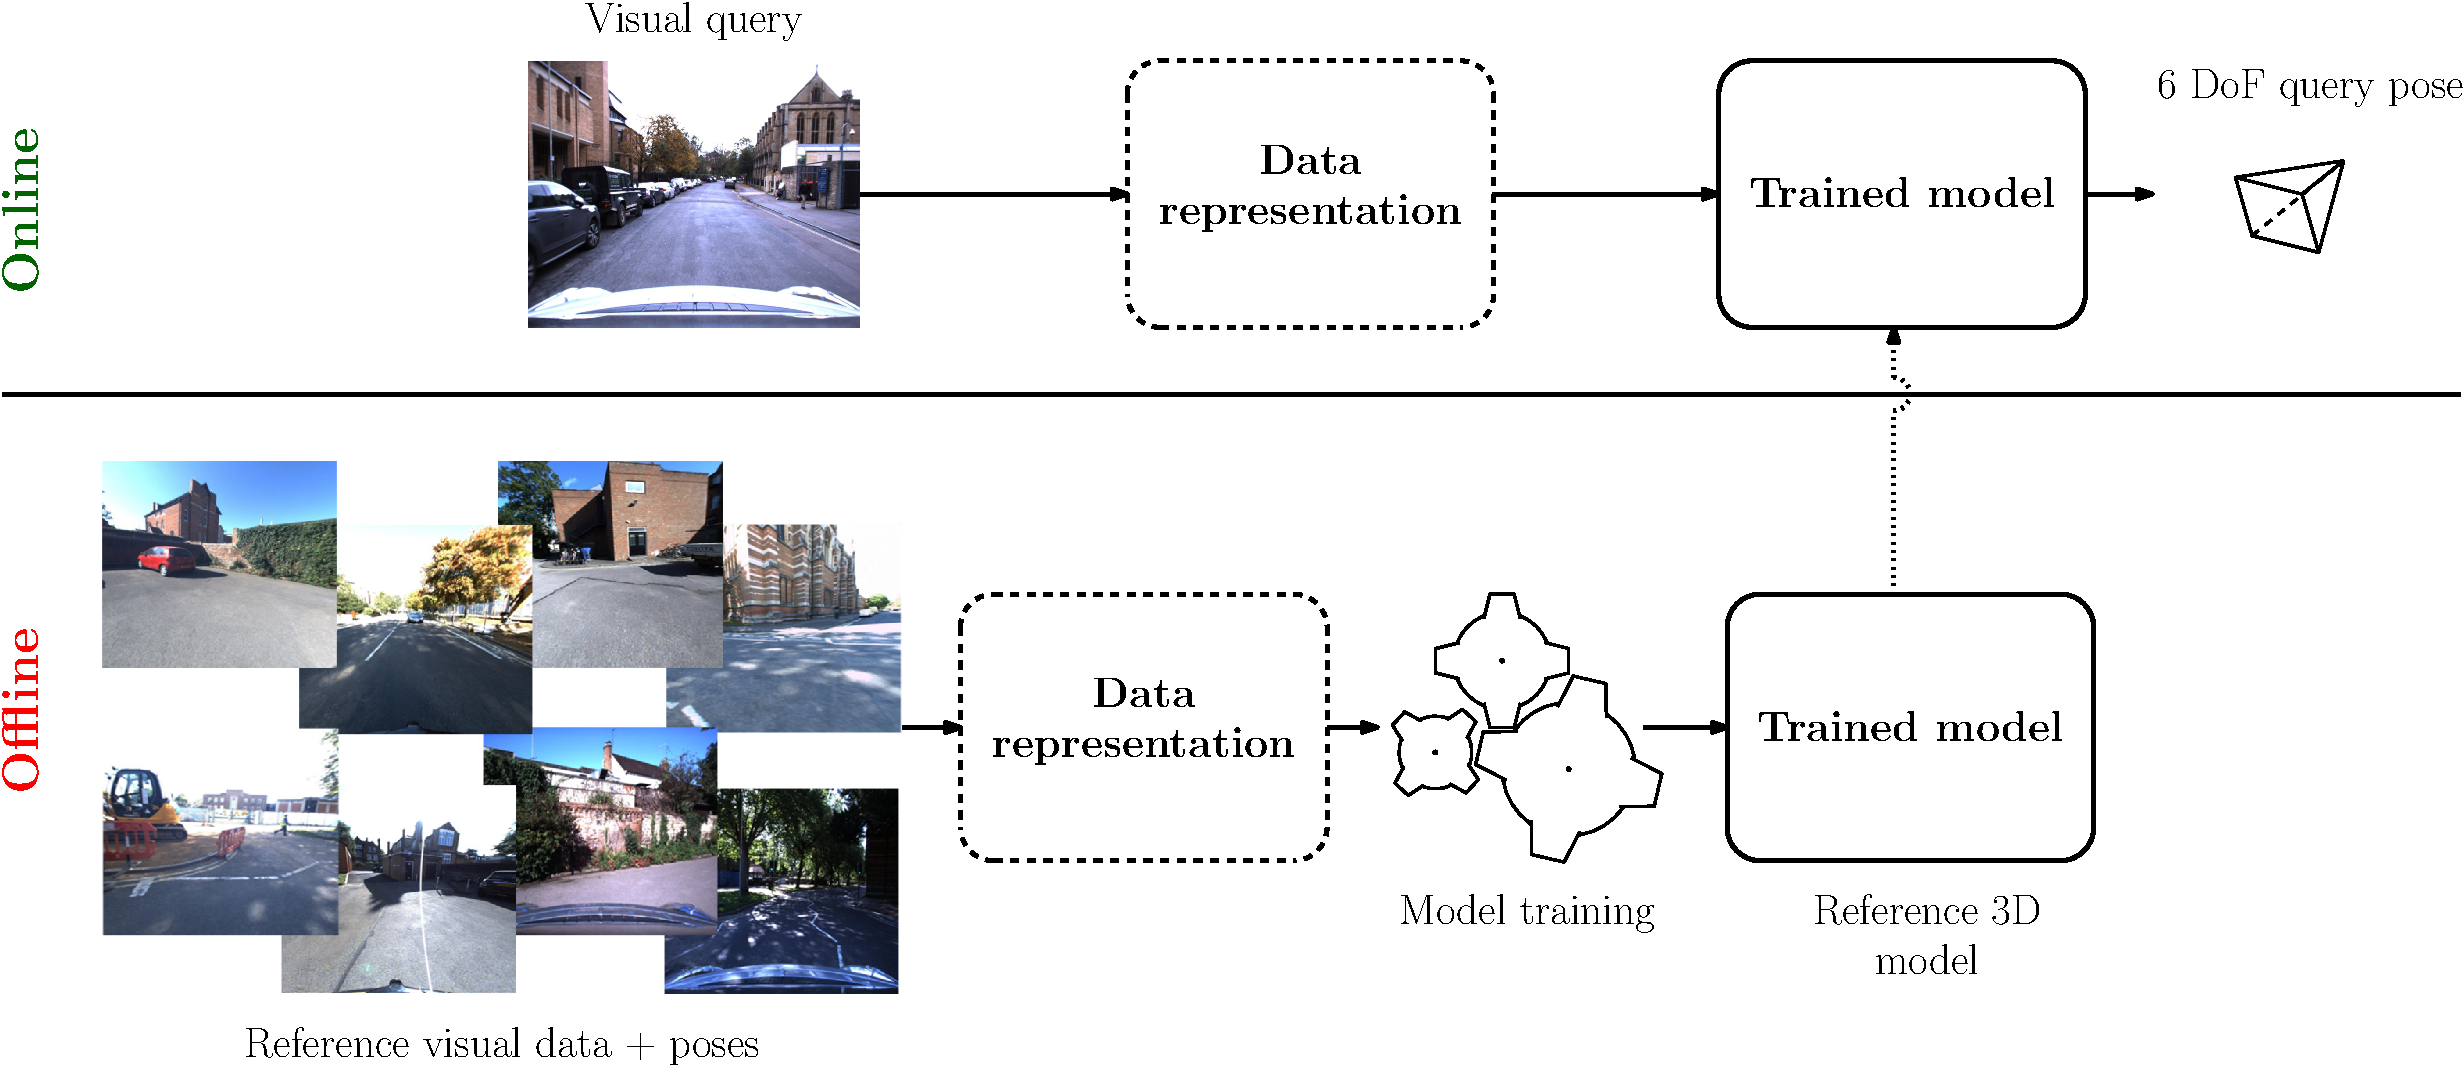
\includegraphics[width=\linewidth]{methods/learned_method}
	\caption[Learned method]{\label{fig:learned_method}\textbf{Learned method for \acs{vbl}:} a model is trained with geolocalized data in order to regress the right pose of a visual request. Once trained, the model is used to predict the pose of a unknown query. The data can be preprocessed before the evaluation by the model.}
\end{figure}


\label{subsubsec:pose_regression}
The last class of 6-\ac{dof} pose estimation methods cast \ac{vbl} as a pose regression problem. A model is trained with geolocalized visual data in order to be able to predict the 6-\ac{dof} pose of an unknown visual request. Key components of learned methods are presented in figure~\ref{fig:learned_method}. Two different kinds of model are employed in the literature: 
local-based~\citep{Shotton2013} (\eg training samples are pixels in image)

global-based~\citep{Kendall2015} (\eg training samples the raw images).

\paragraph{Local-based learning}
Intro 1 pixel -> 1 3D coord (scene coordinate) 
Training -> query time, 2D/3D -> PnP + RANSAC
Not scalable -> 1 model by scene (only indoor)

In the initial works by~\citet{Shotton2013}, authors encode, thanks to RGB-D data, the global position of each pixel associated to a known environment in a regression forest. At query time, a handful of pixels from a depth camera frame are processed into the regression forest. The multiple pose hypothesis obtained for each pixel is then optimized in a random consensus to regress the camera position and orientation. This method is fast and precise and can be used on texture-less data. However, the depth information associated to each pixel is needed and the authors have to train a specific forest for each 3D scene. This initial method have been improved in~\citep{Guzman-rivera2014}, where authors take in consideration several candidates for the final pose regression obtained by trained predictors. \citet{Valentin2015} introduce mixture of Gaussian to represent the uncertainty associated with the regression forest prediction and significantly improve the 6 \ac{dof} estimation by embedding this information within the full camera pose regression step. The regression forest have been replaced by Neural Network (NN) in~\citep{Massiceti2016}, bringing slightly better result at the cost of computational overhead. \citet{Meng2016} consider only RGB images at query time. The loss in precision is compensated by a post pose refinement step based on nearest neighbors search with sparse extracted SIFT features (like in structured approaches, see section~\ref{subsubsec:sfm_methods}).

Inspired by works presented above, \citet{Glocker2013} (extended version in~\citep{Glocker2015}) design a system based on regression ferns to quickly associate an RGB-D image to a binary feature. Ferns produce descriptor according to randomly initialized binary rules, and a look up table is maintained to directly associated image signature with 3D pose in the scene. Presented system is less precise that the one presented by~\citet{Shotton2013} but has the advantages of not relying on a heavy pre-processing step (\ie the spawning of the regression forest). Along the same line, \citet{Cavallari, Cavallari2018} propose a new method based on pre-trained regression forest. This method permit to recover the pose of a RGB-D camera without prior knowledge about the 3D scene, more precisely than~\citet{Glocker2013,Glocker2015}. 

\citep{Brachmann2017b} -> deep feature extraction before coordinate localization + DSAC~\citep{Brachmann2017}. Loss improvement~\citep{Li2018}

\citep{Cavallari2019}: idea (pose reservoir) from applied with \citep{Brachmann2017b} fully convolutional model

Hybrid~\citep{Duong2018} (patch -> coord)

\paragraph{Global-based learning}
\label{para:cnn_regressor}

1 image -> 1 6-\ac{dof} pose

Introduced in 2015 by \citet{Kendall2015}, PoseNet consists of the fine-tuning of a \ac{cnn} for the task of localization. The network is trained upon a set of paired image/pose and automatically regress the 6 \ac{dof} pose of a camera that acquired a colour image. The pose obtained through this method is not as accurate as the pose obtained with ``classical'' direct methods \citep{Feng2016a,Sattler2016a} but provide great tolerance to changes in scale and appearance. Compared to regression forest~\citep{Valentin2015}, \ac{cnn} seems more appropriate to handle large environment and does not rely on depth information.

Recent improvement have been proposed by the original authors~\citep{Kendall2016} to integrate an uncertainty estimation in the regression process. \citet{Liu2016} integrate this \ac{cnn} architecture with only depth map information for recovering the pose of a camera in complete obscurity. The work by Walch et al.~\citep{Walch2016mastersThesis,Walch2016a} present a combination of a PoseNet~\citep{Kendall2015} with a \ac{lstm} units plugged at the output of the network in order to encode stronger spatial information from the image. This combination slightly improves the precision of the system. \citet{Jia2016} highlight the limited number of training example available for \ac{cnn} pose regressors. Though the learning transfer seems to be efficient~\citep{Kendall2015}, authors propose a new method to gather supplementary image/pose pairs for the fine-tuning step. They generate artificial images from a dense point cloud model obtained by \ac{sfm} thanks to a rendering software. Computer graphics shaders effects are added on some rendered views for simulating various illuminations. \citet{Contreras2017} exploit this CNN architecture in order to create a fixed size map that can be improved by adding new trajectories. Authors were able to reduce the original size of the CNN by factor of three while maintaining similar localization performances on indoor scenes. Recent contribution~\citep{Kendall2017} investigate new loss-functions for the training phase of the \ac{cnn}, by adding constraints from multi-view geometry standards~\citep{Hartley2003}.

Although Posenet has the advantages of being lightweight and relies on only-images data, \citet{Sattler2019} show that performances of such methods are less precise than CBIR-based pose estimation (section~\ref{subsec:vbl_as_image_retrieval}). They demonstrate that learned pose regression method are more likely to average the pose of the training examples~\citep{Torii2013} rather that computing a real pose based on geometric constraints. Another disadvantage of Posenet-like methods rely on the fact that a different model has to be trained for each new scene.

Differently, recent work from~\citet{Weyand2016} consider the localization problem as a classification task. They perform a worldwide training on 126M images categorized into 26k places across the globe. According to a given image a \ac{cnn}, named PlaNET, estimates a map of probable location for the query. Localization of multiples photos taken from a common album can be performed by augmenting the original network with a \ac{lstm} layer. \citet{Vo2017} push further the study of such a neural network and conclude that the features extracted from layers of PlaNET are more discriminative to determine the location of an input image that the CNN classifier itself. By extracting features instead of using a classification algorithm, their contribution is closer to the original world-wide localization method IM2GPS~\citep{Hays2008}. CPlanet~\citep{Seo2018}

\subsection{Coarse to fine localization}

As our second principal contribution in this thesis is a new coarse to fine 6-\ac{dof} pose estimation method, we review state of the art of these type of methods in chapter~\ref{chap:4}.
